\chapter{Анализ масштабируемости, параллельной эффективности и ускорения параллельной ВС}
			%	ОБЩЕЕ ПРАВИЛО ДЛЯ ВТОРОЙ ГЛАВЫ: НЕ ПЛАНРИРОВАТЬ ЧТО_ТО НОВОЕ И ОЧЕНЬ ХОРОШЕЕ ЧЕГТО НЕТ, А ПОДКРЕЛЯТЬ И УИСИЛВАТЬ ТО, ЧТО РЕАЛЬНО ЕСТЬ.
			%	ЕСЛИ У НАС СЛАСБОСТЬ В ОБЛАСТИ АНАЛИЗА КОММ СТРУКТУРЫ - НУ И ЛАДНО, И ПУСТЬ ОНА БУДЕТ. ГОВОРИТЬ БОЛЬШЕ О МАСШТАБИРУЕМОСТИ. А КОРММ СТРУКТУРУ АНАЛИЗИРПОВАТЬ ЧЕРЕЗ ПЕРЕСЫЛКИ ЧАСТИЦ
			%	НАША ИДЕЯ не ПОДМЕНЯТЬ СОБОЙ ДИАГНОСТИКУ АРХИТЕКТУРЫ, а мерять И ОПРЕДЕЛЯТЬ ВСЕ ЧЕРЕЗ ИЗМЕРЕНИЯ ВРЕМЕН ПО PIC
				В четвертой главе предложена методика интегральной оценки тестируемой ВС с помощью измерения масштабируемости с расчетах по методу частиц в ячейках и определения на основе измерений возрастания потока данных в коммуникационной сети ВС.
%				На основе данных о пересылке модельных частиц измерена производительность коммуникационной сети ВС, при этом важно отметить преимущества использованного метода измерений: пересылка данных имеет высокую степень нерегулярности, а также большой объем, что означает проведение тестирования на большой нагрузке, и возможность широкого применения полученных таким образом данных.
%				Также предложена и апробирована методика определения фактически соседних (с точки зрения MPI) узлов ВС.  
							
			\section{Определение понятий эффективности, масштабируемости и ускорения}
			%\textbf{Степаненко, книжка"высокопроизводительные вычисления", учебник Воеводина}
			
			Выписано определение эффективности параллельной реализации программ, сильной и слабой масштабируемости, ускорения при распараллеливании.
			
			В частности, ускорение параллельного алгоритма для $N$ процессоров, определяется как:
			$$
			S_N = \frac{T_1(n)}{T_N(n)}
			$$  
			здесь $T_1$ - время исполнения алгоритма на одном процессоре, $T_N$ - на $N$ процессорах, величина $n$ характеризует вычислительную сложность решаемой задачи, для определения ускорения существенно, что задачи, решаемые на 1 и на $N$ процессорах имеют одинаковую сложность.
			Далее, эффективность распараллеливания вычисляется как
			$$
			\eta_N = \frac{1}{N}\frac{T_1(n)}{T_N(n)}
			$$  
			эта величина иногда называется эффективностью в сильном смысле (англ. strong efficiency). Кроме того, часто используется эффективность в слабом смысле (англ. weak efficiency):
			\begin{equation}
			\label{weak_eff}
			\eta^{weak}_N = \frac{T_1(1)}{T_N(N)}
			\end{equation}
			здесь, в отличие от определения ускорения, задачи, решаемые на одном и на $N$ процессорах, имеют различную сложность, т.е. при увеличении количества процессоров в $N$ раз сложность задачи такжэе увеличивается в $N$ раз, и таким образом определяемая эффективность будет 100 \% в том случае, если время вычислений не возрастает при увеличении сложности задачи пропорциональном увеличению количества процессоров.   
			
			Приведены различные используемые варианты этих определений, перечислены факторы, влияющие на  значения этих величин для конкретной ВС, а именно скорость обмена данными и структура коммуникационной сети ВВС, алгоритмы реализации MPI-процедур, в особенности коллективных, настройки коммуникационной системы (таймауты, размер системных буферов, и др.).
			%\textbf{написать формулы} 
			%\textbf{привести формулы из статьи в СибЖВМ}
			Для последующего анализа измереннного времени работы метода частиц в ячейках на параллельной ВС, и для прояснения зависимости этого времени от параметров расчета можно привести следующую схематическую формулу для длительности одного временного шага, аналогично статье (Вшивков В.А. и др., СибЖВМ, 2003):
			
			\begin{equation}
			\label{PIC-timestep}
			T=T_{F} \left ( \frac{N_x N_y N_z }{P_E}\right )+ T_{F,S}\left (N_y N_z\right ) + T_P\left(\frac{N_p}{P_E\times P_L}\right) +T_{P,S}\left (\frac{N_p*T_p}{P_E\times P_L}\right)
		\end{equation}
			 
		здесь $T_{F}$ - время вычисления электромагнитного поля, $N_x, N_y, N_z$ - размер расчетной сетки соответственно, по координатам $X$ $Y$ и $Z$, $P_E$ - количество процессоров для эйлеровой декомпозиции, т.е. для разделения расчетной области на подобласти, $T_{F,S}$ - время, затрачиваемое на персылку граничных значений полей и токов между подобластями, которое зависит только от $N_y$ и $N_z$ в силу того что на данный момент используется одномерная декомпозиция,  $T_P$ - время расчета движения частиц, $P_L$ - количество процессов (или потоков) для лагранжевой декомпозиции, т.е. для дополнительного разделения частиц подобласти на группы, вычисляемые на отдельных ядрах.
		
		

		
		
		\section{Анализ масштабируемости как интегральной характеристики ВС.}
		
		Во втором разделе приведены фактически измеренные на различных высокопроизводительных ВС графики масштабируемости и параллельной эффективности и на основе этих данных проведен анлиз коммуникационной сети данных ВС, в частности, для МВС-100К, рис. \ref{eff2}. 
		
		\begin{figure}[h]
			\begin{center}
				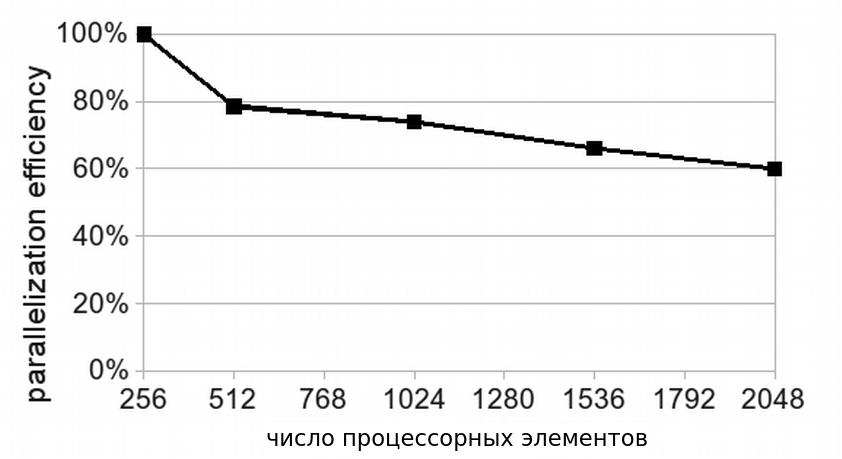
\includegraphics[height=5cm,keepaspectratio]{images/eff_weak_JSCC.png}
				\caption{
					Эффективность распараллеливания в слабом смысле, для МВС-100К, МСЦ РАН.
				}
				\label{eff2}
			\end{center} 
		\end{figure}
		
		Возможность проведения анализа коммуникационной сети с помщью расчетов по методу частиц в ячейках основана на известной информации о количестве пересылаемых данных и о виртуальной топологии, используемой в программе.
		
		Размер данных, перемещаемых между двумя соседними MPI-процессами равен $144 \times N_y N_z  $ байт. При этом в идеальном случае, когда соседние MPI-процессы находятся на соседних узлах, коммуникации происходят только между соседними узлами, и поток данных в системе в целом не возрастает с ростом количества используемых в расчете узлов.
		
		В частности, в расчете показанном на рис. \ref{eff2} использована эйлерова декомпозиция. Это означает, что используются только парные пересылки MPI, коллективные пересылки не используются, и поток данных через коммуникационную систему ВС в целом возрастать не должен. Если, тем не менее, он возрастает, что видно на рис. \ref{eff2} в виде снижения эффективности распараллеливания, то это может (при отсутствии коллективных операций), означать, что соседние с точки зрения MPI процессы находятся на физически удаленных друг от друга узлах параллельной ВС.
		
		Обозначая $k_{||}$ зависимость коэффициента при времени пересылок граничных условий от количества процессоров в формуле \ref{PIC-timestep}, так что 
		\begin{equation}
		T_{F,S} = k_{||} (P_E) \frac{N_y N_z}{P_E}
		\end{equation} 
		и подставляя формулу \ref{PIC-timestep} d \ref{weak_eff}, рассматривая только лишь время расчета и пересылок электромагнитного поля, можно получить 
		\begin{equation}
		k_{||} (P_E) = \frac{1}{\eta^{weak}(P_E)} - 1
		\end{equation}	  
		Таким образом величина $k_{||} (P_E)$  - \textbf{степень нелинейности} коммуникационной структуры параллельной ВС. Фактически она представляет собой отклонение от линейной функции для зависимости времени пересылок от количества процессоров. Он показывает предел возрастания потока данных через коммуникационную структуру ВС при увеличении количества процессоров, используемых в расчете. Эта величина характеризует, в какой степени при передаче информации между соседними процессами в MPI используются узлы параллельной ВС, не являющиеся ближайшими соседями. В силу того, что на значение эффективности оказывает влияние не только свойства оборудования, но и особенност реализации MPI, возникает необходимость разделить эти факторы. Это достигается с помощью привязки процессорв к узлам. 
		
		В итоге, такимобразом определенная  величина $k_{||} $ может быть использована как характеристика параллельной ВС, показывающая реально достижимую с помощью данной ВС эффективность и масштабируемость   
		
		\subsection{Измерение продолжительности параллельных коммуникаций и анализ характеристик и топологии коммуникационного оборудования}
		Здесь описано решение задачи об определении соседства процессов по реальным узлам. Это исключительно важно для производительности реальных задач, чтобы виртуально близкие (т.е. по номеру MPI-процесса) процессы исполнялись бы на соседних узлах многопроцессорной ВС. Для этого проводится обмен сообщениями между узлами, выделенными 
		для исполнения программы по топологии полного графа, и проводится анализ времени прохождения сообщений, рис. \ref{poly_all2all}.  
		
		Следует отметить, что такого этапа, с обменом сообщениями между всеми процессами в рамках метода частиц нет, поэтому, такой анализ проводится предварительно, перед запуском основной части программы.

		
		\begin{figure}[htb]
			\begin{center}
				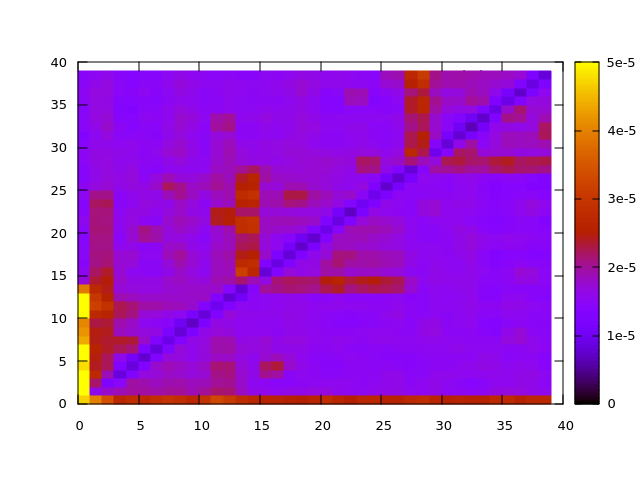
\includegraphics[height=7cm,keepaspectratio]{images/polytech_all_to_all.png}
			\end{center}
			\caption{Время пересылок для 40 MPI-процессов, расположенных на 10 узлах по 4 процесса, кластер «Политехник», СПбПУ. По осям X и Y отложены номера процессов, цветовая шкала показывает время пересылок в секундах.}
			\label{poly_all2all}
		\end{figure} 
		Узлы с минимальным временем считаются близкими, т.е. выясняется фактическая топология ВС. Это сопоставляется с известной информацией о размещении процессов по узлам.	Для повышения производительности приложения в дальнейшем целесообразно передвинуть соседние процессы на те узлы, где по факту меньше задержка по коммуникациям.
		
		%	\textbf{картинку из стьатьи все-со-всеми, (с Политеха)}. 
		%	1.измерение всех видов MPI-коммуникаций, сравнение одного с другим (Send, Isend, Bsend) - и увязатиь это с алгоритмом
		%	2. варьирование размера сообщений и пр. параметров
		
		\textbf{материал статьи НГУ ИТ  с более аакуратным анализом}

		\subsubsection{Измерение производительности коммуникационной сети на основе данных о пересылке модельных частиц}
		В \textit{четвертом разделе} приведены результаты измерения скорости пересылок модельных частиц в методе частиц в ячейках и проведенный на основе этого сравнительный анализ скорости работы коммуникационной сети ВС.
		
		На нескольких параллельных ВС были измерены времена, затраченные на пересылку модельных частиц между соседними узлами. Из статитики расчетов по методу частиц в ячейках известно, что пересылается, как правило, не более 5\% модельных частиц. В рассматриваемых расчетах размер сетки $512\times 64 \times 64$ узла  при 150 модельных частицах в ячейке, т.е.  на каждом временном шаге в среднем пересылается 15.7 млн. модельных частиц, что при размере одной частицы в 48 байт означает 720 Мб на каждый временной шаг, что при известном времени пересылки позволяет вычислить скорость. Таким образом была экспериментально измерена величина $T_{P,S}$, входящая в формулу \ref{PIC-timestep}   
			
			\begin{figure}[htb]
				\begin{center}
					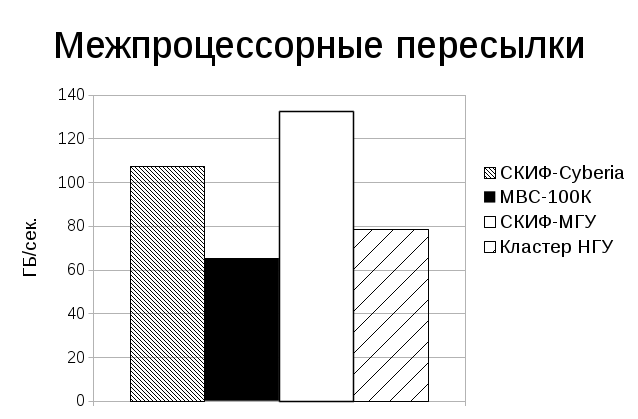
\includegraphics[height=7cm,keepaspectratio]{images/particle_send_GBsec.png}
				\end{center}
				\caption{Скорость пересылки данных на некоторых кластерах. Количество модельных частиц: 2.5 млн. на каждое процессорное ядро. Измерения выполнены в 2010 г.}
				\label{procs_flops}
			\end{figure}
			
			Измеренная таким образом скорость пересылки данных показывает фактический предел этой величины, реально достижимый для вычислительного приложения с использованием имеющегося оборудования и коммуникационного программного обеспечения. Это подтверждается следующими соображениями:
			\begin{itemize}
				\item Объем пересылаемых данных мал: в среднем 6 Мб на процесс
				\item Соседние MPI-процессы, как правило, расположены на близких узлах.
			\end{itemize}  	 
			
		%	\subsubsection{Экстраполяция результатов тестирования ускорения и эффективности распараллеливания}
			%%	формулы из статьи НГУ-ИТ'17, адаптированные и улучшенные, сравнение со Степаненко
			%%	выводы по большой системе на тех же принципах, совпадение с реальностью
			%%	
			%	В \textit{четвертом разделе} описана оригинальная методика экстраполяции результатов на системы большой размерности и ее сравнение с аналогиными работами.Проведено большое количество физических расчетов с использованием программы в трехмерной расчетной области, использующей двухступенчатую эйлерово-лагранжеву декомпозицию расчетной области.На основании тестовых расчетов на небольшом количестве процессорных ядер измереятся время коллективных и парных коммуникаций MPI и строится аппроксимацию времени пересылок для произвольного количества процессов.
			
			%	Основным вопросом является соответствие реально измеряемого времени выполнения коммуникационных операций для определенного количества процессоров, 
			%	 По результатам вырабатываются рекомендации по выбору оптимального сочетания эйлеровой и лагранжевой декомпозиции.
			%	\textbf{формулы}
			
			%	\subsection{Глава 3: Анализ производительности системы памяти}
			%	\subsubsection{Кэш-память}    
			%	Статьи PACO (кэш, списки и пр.), BOE (данны исполения на Sun Sparc Opteron)
			%	\subsubsection{Оперативная память}
			%	 PAVT10, Абрау7 PACO